\documentclass[12pt, a4paper]{article}

\newcommand*{\Author}{Roberto Gesteira Miñarro}
\newcommand*{\Keywords}{Red neuronal, árbol de decisión, clustering, reglas de asociación}
\newcommand*{\Subject}{Detección de Phishing}
\newcommand*{\Title}{Detección de phishing}

\usepackage{amsmath}
\usepackage{amssymb}
\usepackage[spanish, es-nodecimaldot]{babel}
\usepackage[font=small, labelfont=bf, labelsep=period]{caption}
\usepackage{csquotes}
\usepackage{datetime}
\usepackage{float}
\usepackage[T1]{fontenc}
\usepackage[bmargin=3cm, lmargin=3cm, rmargin=3cm, tmargin=3cm]{geometry}
\usepackage{graphicx}
\usepackage[breaklinks]{hyperref}
\usepackage[utf8]{inputenc}
\usepackage[newfloat]{minted}
\usepackage{multicol}
\usepackage{parskip}
\usepackage{siunitx}
\usepackage{titletoc}
\usepackage{xcolor}

\renewcommand{\textit}{\textsl}

\colorlet{bgcolor}{gray!10}

\newcommand{\itab}[1]{\hspace{0em}\rlap{#1}}
\newcommand{\tab}[1]{\hspace{.14\textwidth}\rlap{#1}}

\titlecontents{figure}[0em]{}{\itab{\textbf{\figurename~\thecontentslabel.}} \tab{\ }}{}{\titlerule*[0.8pc]{.}\contentspage\vspace{8pt}}[]

\providecommand{\sectionname}{Sección}

\addto\captionsspanish{\renewcommand{\contentsname}{Índice de la memoria\newline}}
\addto\captionsspanish{\renewcommand{\figurename}{Figura}}
\addto\captionsspanish{\renewcommand{\listfigurename}{Índice de figuras\newline}}

\newcommand*{\figref}[1]{\figurename~\ref{fig:#1}}
\newcommand*{\sectionref}[1]{\hyperlink{sec:#1}{\sectionname~{#1}}}

\hypersetup{
  colorlinks=true,
  linkcolor=black,
  pdfauthor=\Author,
  pdfkeywords=\Keywords,
  pdfsubject=\Subject,
  pdftitle=\Title,
  urlcolor=blue
}
\urlstyle{same}

\graphicspath{{./images/}}

\newcommand{\figcaption}[4][H]{
  \begin{figure}[#1]
    \centering
    \includegraphics[width=#4\textwidth]{#2}
    \caption{#3}
    \label{fig:#2}
  \end{figure}
}

\newcommand*{\sourcedir}{../src}

\usemintedstyle{vs}

\newcommand*{\codebgnocaption}[3][fontsize=\scriptsize, linenos=false]{
  \begin{listing}[H]
    \inputminted[bgcolor=bgcolor, #1]{#3}{\sourcedir/#2}
  \end{listing}
  \vspace{-1.2cm}
}

\newcommand*{\cluster}{\textit{cluster}}
\newcommand*{\clusters}{\textit{clusters}}
\newcommand*{\clustering}{\textit{clustering}}
\newcommand*{\Clustering}{\textit{Clustering}}
\newcommand*{\dataset}{\textit{dataset}}
\newcommand*{\kmeans}{\textit{K-means}}
\newcommand*{\ML}{\textit{Machine Learning}}
\newcommand*{\phishing}{\textit{phishing}}
\newcommand*{\script}{\textit{script}}
\newcommand*{\Script}{\textit{Script}}

\title{\underline{\textbf{Detección de \phishing}}}
\author{\Author}
\newdate{date}{27}{05}{2021}
\date{\displaydate{date}}

\begin{document}

  \vspace{3cm}
  \maketitle

  \newpage
  \tableofcontents

  \newpage
  \listoffigures

  \newpage
  \section*{Introducción}
    \addcontentsline{toc}{section}{Introducción}

    En este trabajo se realiza un análisis de un \dataset\ con características de URL accesibles por HTTP o HTTPS mediante distintos algoritmos de \ML\ conocidos.

    El \dataset\ utilizado puede encontrarse en \url{https://www.kaggle.com/manishkc06/web-page-phishing-detection}, aunque el contenido original está en \url{https://data.mendeley.com/datasets/c2gw7fy2j4/2}, junto con algunos códigos de Python para obtener las características de cada URL.

    El objetivo del análisis es obtener distintos modelos que puedan predecir si una URL contiene algún tipo de \phishing\ en base a las propias características de la URL, principalmente. El desarrollo de los modelos y su análisis se realiza en R.

    Como solución adicional, se pretende elaborar una herramienta que, dada una URL, pueda detectar si es legítima o contiene \phishing. Para ello, en primer lugar se caracteriza la URL con un \script\ de Python (adaptado de los obtenidos junto al \dataset); y en segundo lugar, se introducen estas características al modelo creado con R para predecir el tipo de URL.

    De esta manera, sería posible prevenir ataques de \phishing\ integrando esta herramienta en navegadores o clientes de correo electrónico, para analizar una URL y avisar al usuario de un peligro potencial.

  \section{Caracterización y exploración del \dataset}

    En primer lugar, es necesario visualizar el \dataset\ para conocer las variables que hay involucradas y el número de ejemplos disponibles.

    El \dataset\ inicial contiene $89$ variables y $11\,481$ observaciones. Por experiencia, se sabe que con un \dataset\ de este estilo se tardará mucho tiempo en entrenar los modelos (sobre todo con algoritmos de \clustering). Por este motivo, es necesario realizar una limpieza del \dataset.

    De las $89$ variables, hay $6$ que tienen siempre el mismo valor para todas las observaciones. Es evidente que estas variables no aportan información relevante y que hay que eliminarlas del \dataset.

    Por otro lado, existe una variable que sirve como índice (la propia URL) y la variable de resultado \texttt{status}, que indica si la URL es legítima o contiene \phishing.

    Para determinar si entre las $81$ variables restantes hay alguna más importante que las demás, se realiza un análisis de componentes principales (PCA), obteniendo el siguiente \textit{scree plot}:

    \figcaption{pca1.png}{Análisis de componentes principales sobre el \dataset\ original}{1}

    Como se puede ver en la \figref{pca1.png}, no es posible distinguir ninguna componente realmente importante, ya que la barra más alta apenas supera el \SI{10}{\percent}. Entonces, es necesario buscar otro método para disminuir el tamaño del \dataset.

    Puede verse en el \dataset\ que existen variables binarias que tienen el mismo valor para más del \SI{90}{\percent} de los ejemplos, lo cual indica que estas variables no aportan demasiada información, ya que solo destacan en contados ejemplos. Por este motivo, se eliminan primero estos ejemplos y, acto seguido, se elimina la variable (porque todos los ejemplos tendrán el mismo valor).

    El proceso anterior se realiza varias veces hasta que el \dataset\ se estabiliza en $47$ variables (contando \texttt{url} y \texttt{status}) y $5\,445$ observaciones. Ahora, el conjunto de datos es más ligero y permite trabajar mejor.

    De todas maneras, se vuelve a realizar un PCA sobre este conjunto reducido para ver si había alguna componente destacada. A la vista de la \figref{pca2.png}, se concluye que no hay componentes principales.

    Para los siguientes apartados, el \dataset\ que se utiliza es el \dataset\ reducido.

    \figcaption{pca2.png}{Análisis de componentes principales sobre el \dataset\ reducido}{1}

    \subsection{Variables del \dataset}

      Una vez definido el \dataset, conviene saber qué mide cada variable. Algunas de las más llamativas son las siguientes:

      \begin{itemize}
        \item \texttt{url}: Contiene el valor de la URL, como texto.
        \item \texttt{status}: Indica si la URL es legítima o contiene \phishing.
        \item \texttt{length\_url}: Número de caracteres de la URL.
        \item \texttt{nb\_dots}: Número de puntos (caracteres) en la URL.
        \item \texttt{https\_token}: `0' si la URL contiene \texttt{https} y `1' en caso contrario.
        \item \texttt{shortening\_service}: `1' si la URL contiene el nombre de algún acortador de URL conocido y `0' en caso contrario.
        \item \texttt{nb\_hyperlinks}: Número de enlaces presentes en el código HTML de la página web.
        \item \texttt{empty\_title}: `0' si la página web contiene un título en el código HTML (\texttt{<title>John Doe</title>}) y `1' en caso contrario.
        \item \texttt{google\_index}: `0' si la URL aparece en la primera página de Google al buscar la URL y `1' en caso contrario.
        \item \texttt{page\_rank}: Calidad de la página web en una escala del 0 al 10.
      \end{itemize}

  \section{Reglas de asociación}

    En este apartado se tratan de relacionar las variables del \dataset\ para obtener reglas que permitan observar algunas dependencias interesantes entre variables.

    En la \figref{rules.png} se muestran las reglas de asociación resultantes. Por ejemplo, las páginas sin título (\texttt{empty\_title=1}) no se muestran en Google (\texttt{google\_index=1}); al igual que las URL que provienen de un acortador (\texttt{shortening\_service=1}).

    Otras reglas interesantes indican que la URL contiene \phishing\ si la página web no tiene título (\texttt{empty\_title=1}) o si la URL está acortada (\texttt{shortening\_service=1}). Y también que si el dominio de la URL está contenido en un conjunto de marcas conocidas (\texttt{domain\_in\_brand=1}), entonces la URL será accesible por HTTPS (\texttt{https\_token=0}).

    \figcaption{rules.png}{Reglas de asociación obtenidas}{1}

    Para generar estas reglas de asociación se ha utilizado el algoritmo \textit{apriori} y el paquete \texttt{arules} de R. Las reglas representadas en el grafo de la \figref{rules.png} tienen una confianza mayor al \SI{50}{\percent}, una cobertura menor que la unidad y están formadas por dos elementos (no existen reglas que involucren más de dos elementos).

    Como el algoritmo \textit{apriori} requiere de variables categóricas, se han utilizado solamente las variables binarias del \dataset, transformadas a tipo factor. A pesar de haber quitado información, las reglas obtenidas tienen explicación lógica y, por tanto, son relevantes.

  \section{\Clustering}

    En este apartado se realizan varios análisis de \clustering. En primer lugar, \clustering\ jerárquico sobre las variables del \dataset\ y posteriormente sobre las observaciones; y, en segundo lugar, \kmeans\ sobre las observaciones. Cabe mencionar que estos algoritmos son no supervisados, es decir, los modelos no saben cuál tiene que ser el resultado.

    \subsection{\Clustering\ jerárquico sobre las variables}

      En primer lugar, se realiza un análisis de \clustering\ jerárquico sobre las variables para verificar su similitud. Después de normalizar el \dataset, se obtiene la siguiente \figref{dist_var.png}, que representa por colores las distancias entre variables según la métrica euclídea:

      \figcaption{dist_var.png}{Distancias entre las variables del \dataset}{1}

      Puede verse que hay dos grupos claramente diferenciados: un grupo con las variables cuya distancia es menor y otro grupo con las variables cuya distancia es mayor. Esto se muestra en el siguiente dendrograma obtenido de realizar un \clustering\ jerárquico de tipo aglomerativo (utilizando el paquete \texttt{agnes} de R y el método de Ward):

      \figcaption{dend_var.png}{Dendrograma de las variables del \dataset}{1}

      En el grupo de color azul se encuentran variables continuas o discretas con varios valores posibles (como \texttt{avg\_word\_path} o \texttt{nb\_dots}), mientras que en el grupo naranja las variables son mayoritariamente binarias (como \texttt{https\_token} o \texttt{google\_index}).

      El análisis realizado sirve para comprender mejor la naturaleza de las variables del \dataset\ y observar similitud entre las mismas. Se realizó también un \clustering\ de tipo divisivo, pero no producía un dendrograma tan claro como el de la \figref{dend_var.png}.

    \subsection{\Clustering\ jerárquico sobre las observaciones}

      En este punto, se realiza un \clustering\ jerárquico sobre los ejemplos del \dataset. En primer lugar, se calcula cuál es el mejor método de \clustering\ aglomerativo para realizar el modelo. Como se puede ver a continuación, el método que obtiene el mejor coeficiente de aglomeración es el método de Ward:

      \begin{minted}[bgcolor=bgcolor]{text}
  average      single    complete        ward
0.9163371   0.8693480   0.9429070   0.9957265
      \end{minted}

      El dendrograma obtenido con este método es el que se muestra en la \figref{ward.png}. Parece que lo más razonable es seleccionar $3$ grupos, los cuales están marcados con colores en la propia gráfica.

      \figcaption{ward.png}{Dendrograma obtenido con \clustering\ aglomerativo y método de Ward}{1}

      A continuación, se compara este modelo con uno de \clustering\ divisivo. El resultado de este segundo modelo es el siguiente dendrograma:

      \figcaption{diana.png}{Dendrograma obtenido con \clustering\ divisivo}{1}

      \newpage

      En este caso es más difícil distinguir grupos, aunque parece que $3$ sigue siendo una buena decisión, como se muestra en la \figref{diana.png}.

      Cabe mencionar que, al tratarse de modelos no supervisados, el resultado obtenido no tiene por qué ser la clase de la URL. De hecho, ambos modelos parecen agrupar el \dataset\ en $3$ grupos, y no en $2$.

      Si se pretende agrupar en $2$ grupos, sabiendo que hay dos tipos de URL en el \dataset, se podrían evaluar los modelos mediante matrices de confusión. Los resultados obtenidos al introducir el mismo \dataset\ con el que se entrenó el modelo, se reflejan en las siguientes matrices de confusión para el método aglomerativo y divisivo, respectivamente:

      \begin{minted}[bgcolor=bgcolor]{text}
             Reference
Prediction   legitimate   phishing
legitimate         2060       1319
phishing           1337        729

             Reference
Prediction   legitimate   phishing
legitimate         2954        425
phishing            888       1178
      \end{minted}

      Como estos resultados no son buenos (precisiones del \SI{51.22}{\percent} y del \SI{75.89}{\percent}), se concluye que este algoritmo no es útil para el objetivo de análisis del \dataset. Además, el modelo tarda un tiempo considerable en entrenarse (más de media hora).

      Como se ha dicho antes, el algoritmo de \clustering\ simplemente realiza grupos en función de la similitud de las observaciones, lo cual no es necesario que coincida con la clase de cada observación.

    \subsection{\kmeans}

      Otro algoritmo de \clustering\ es \kmeans, al cual es necesario indicarle primero el número de \clusters\ para agrupar el \dataset.

      En primer lugar se utiliza el método del codo para ver la evolución del WSS en función del número de \clusters\ $K$, como se muestra en la \figref{elbow.png}.

      En esta gráfica no es posible determinar un número claro de \clusters\ para realizar el algoritmo. Por tanto, se utiliza el método de la silueta para poder escoger $K$. Como se puede ver en la \figref{silhouette.png}, el número $K$ indicado es $2$.

      \figcaption{elbow.png}{Número de \clusters\ según el método del codo}{1}

      \figcaption{silhouette.png}{Número de \clusters\ según el método de la silueta}{1}

      \newpage

      Una vez elegido $K$, se entrena el modelo de \kmeans. Aunque se trata de un modelo no supervisado, se ha utilizado un conjunto de entrenamiento y un conjunto de test, aprovechando que el número de \clusters\ coincide con el número de clases de URL.

      Los resultados obtenidos en matrices de confusión son los siguientes:

      \begin{minted}[bgcolor=bgcolor]{text}
Train:
             Reference
Prediction   legitimate   phishing
legitimate         1970        581
phishing            608        925

Test:
             Reference
Prediction   legitimate   phishing
legitimate          633        195
phishing            201        332
      \end{minted}

      De nuevo, se concluye que \kmeans\ no es un buen método para analizar el \dataset, ya que las precisiones resultantes son del \SI{70.89}{\percent} y del \SI{70.9}{\percent} en entrenamiento y test, respectivamente. Al tratarse de un algoritmo de \clustering, el agrupamiento no tiene por qué coincidir con la clase de la URL.

  \section{Mapas de Kohonen}

    El siguiente análisis a realizar se basa en mapas auto-organizados de Kohonen. Este modelo es un tipo de red neuronal que puede ser supervisado o no supervisado.

    Los parámetros principales de este modelo son el número de neuronas, las dimensiones y la topología del mapa. Tras realizar varias pruebas con distintas dimensiones y topologías, se vio que un modelo se obtenía con una topología hexagonal y dimensiones $3 \times 3$ ($9$ neuronas). Como coeficiente de aprendizaje $\alpha$ se utiliza el que proporciona el algoritmo del paquete \texttt{kohonen} por defecto.

    \subsection{Modelo no supervisado}

      En la \figref{maps.png} se muestra la importancia de cada variable en las neuronas del mapa. Con esto, se puede determinar si hay alguna variable redundante. Por ejemplo, las variables \texttt{longest\_words\_raw}, \texttt{longest\_word\_path}, \texttt{avg\_words\_raw} y \texttt{avg\_word\_raw} son muy similares a la variable \texttt{length\_url}, ya que los mapas obtenidos tienen los mismos colores.

      A continuación, se eliminan las variables redundantes y se vuelve a entrenar el modelo. La importancia de las variables es ahora la que se muestra en la \figref{maps_nr.png}.

      \begin{figure}[H]
        \centering
        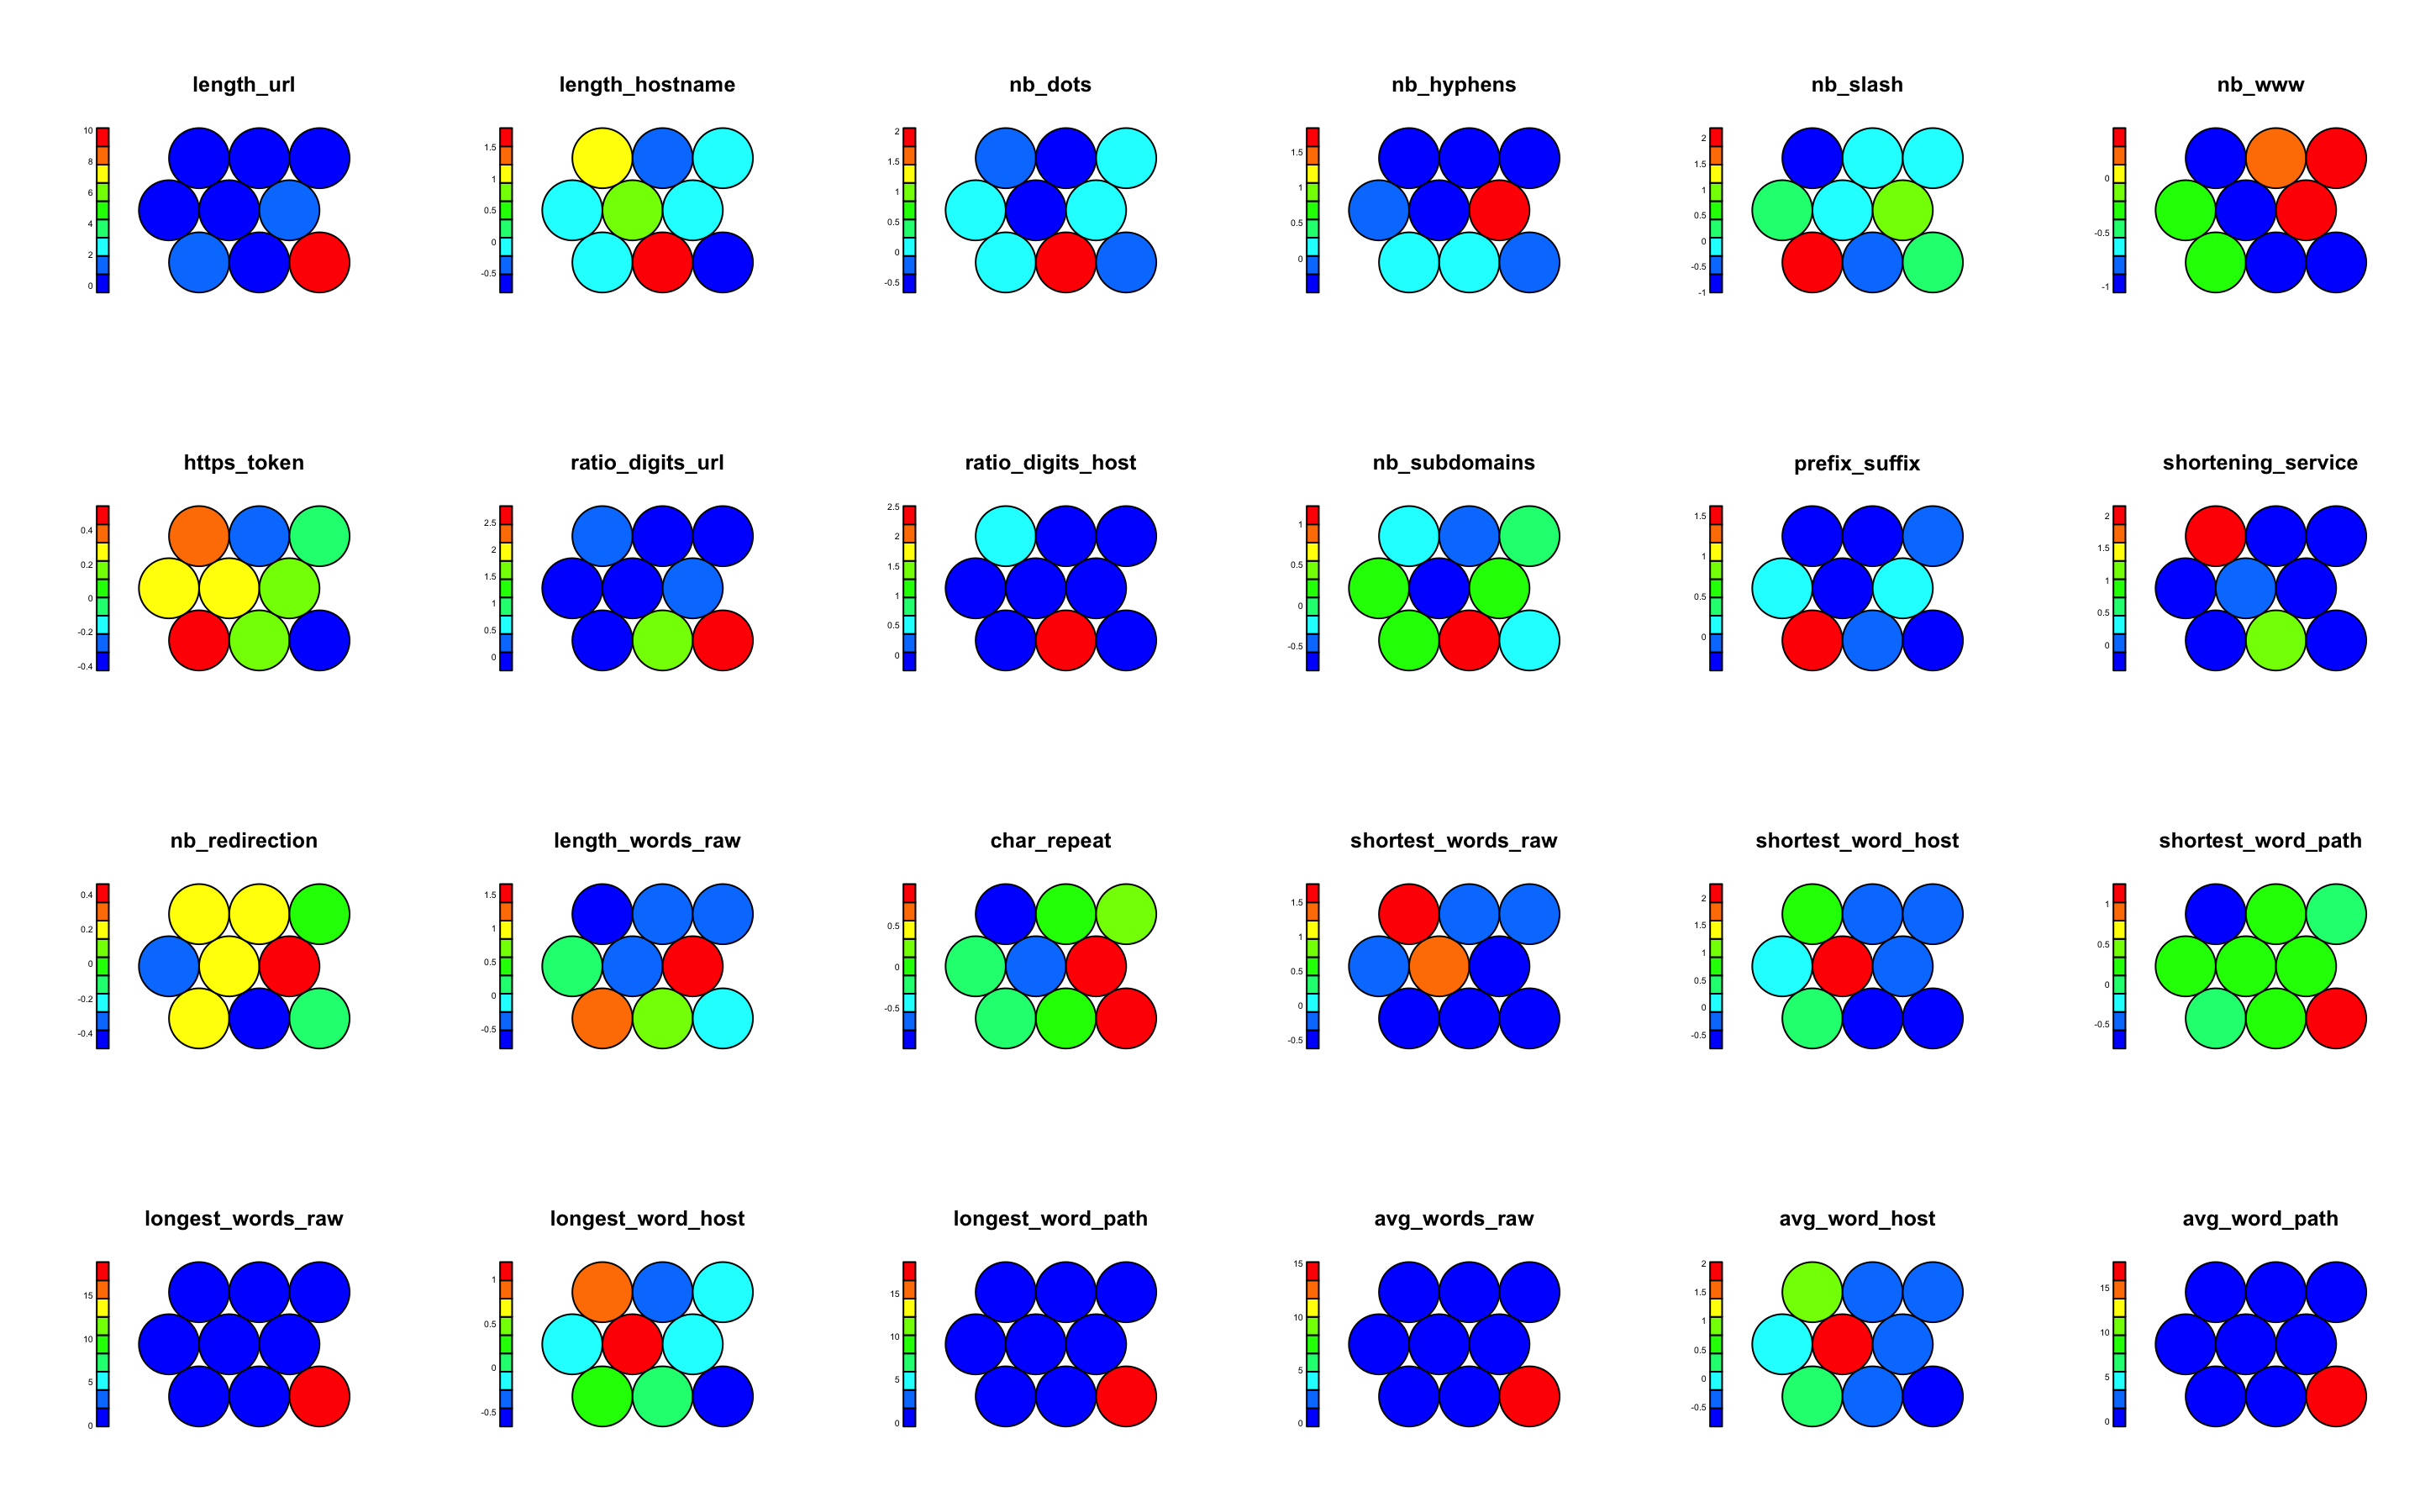
\includegraphics[width=1\textwidth]{maps1.png}
        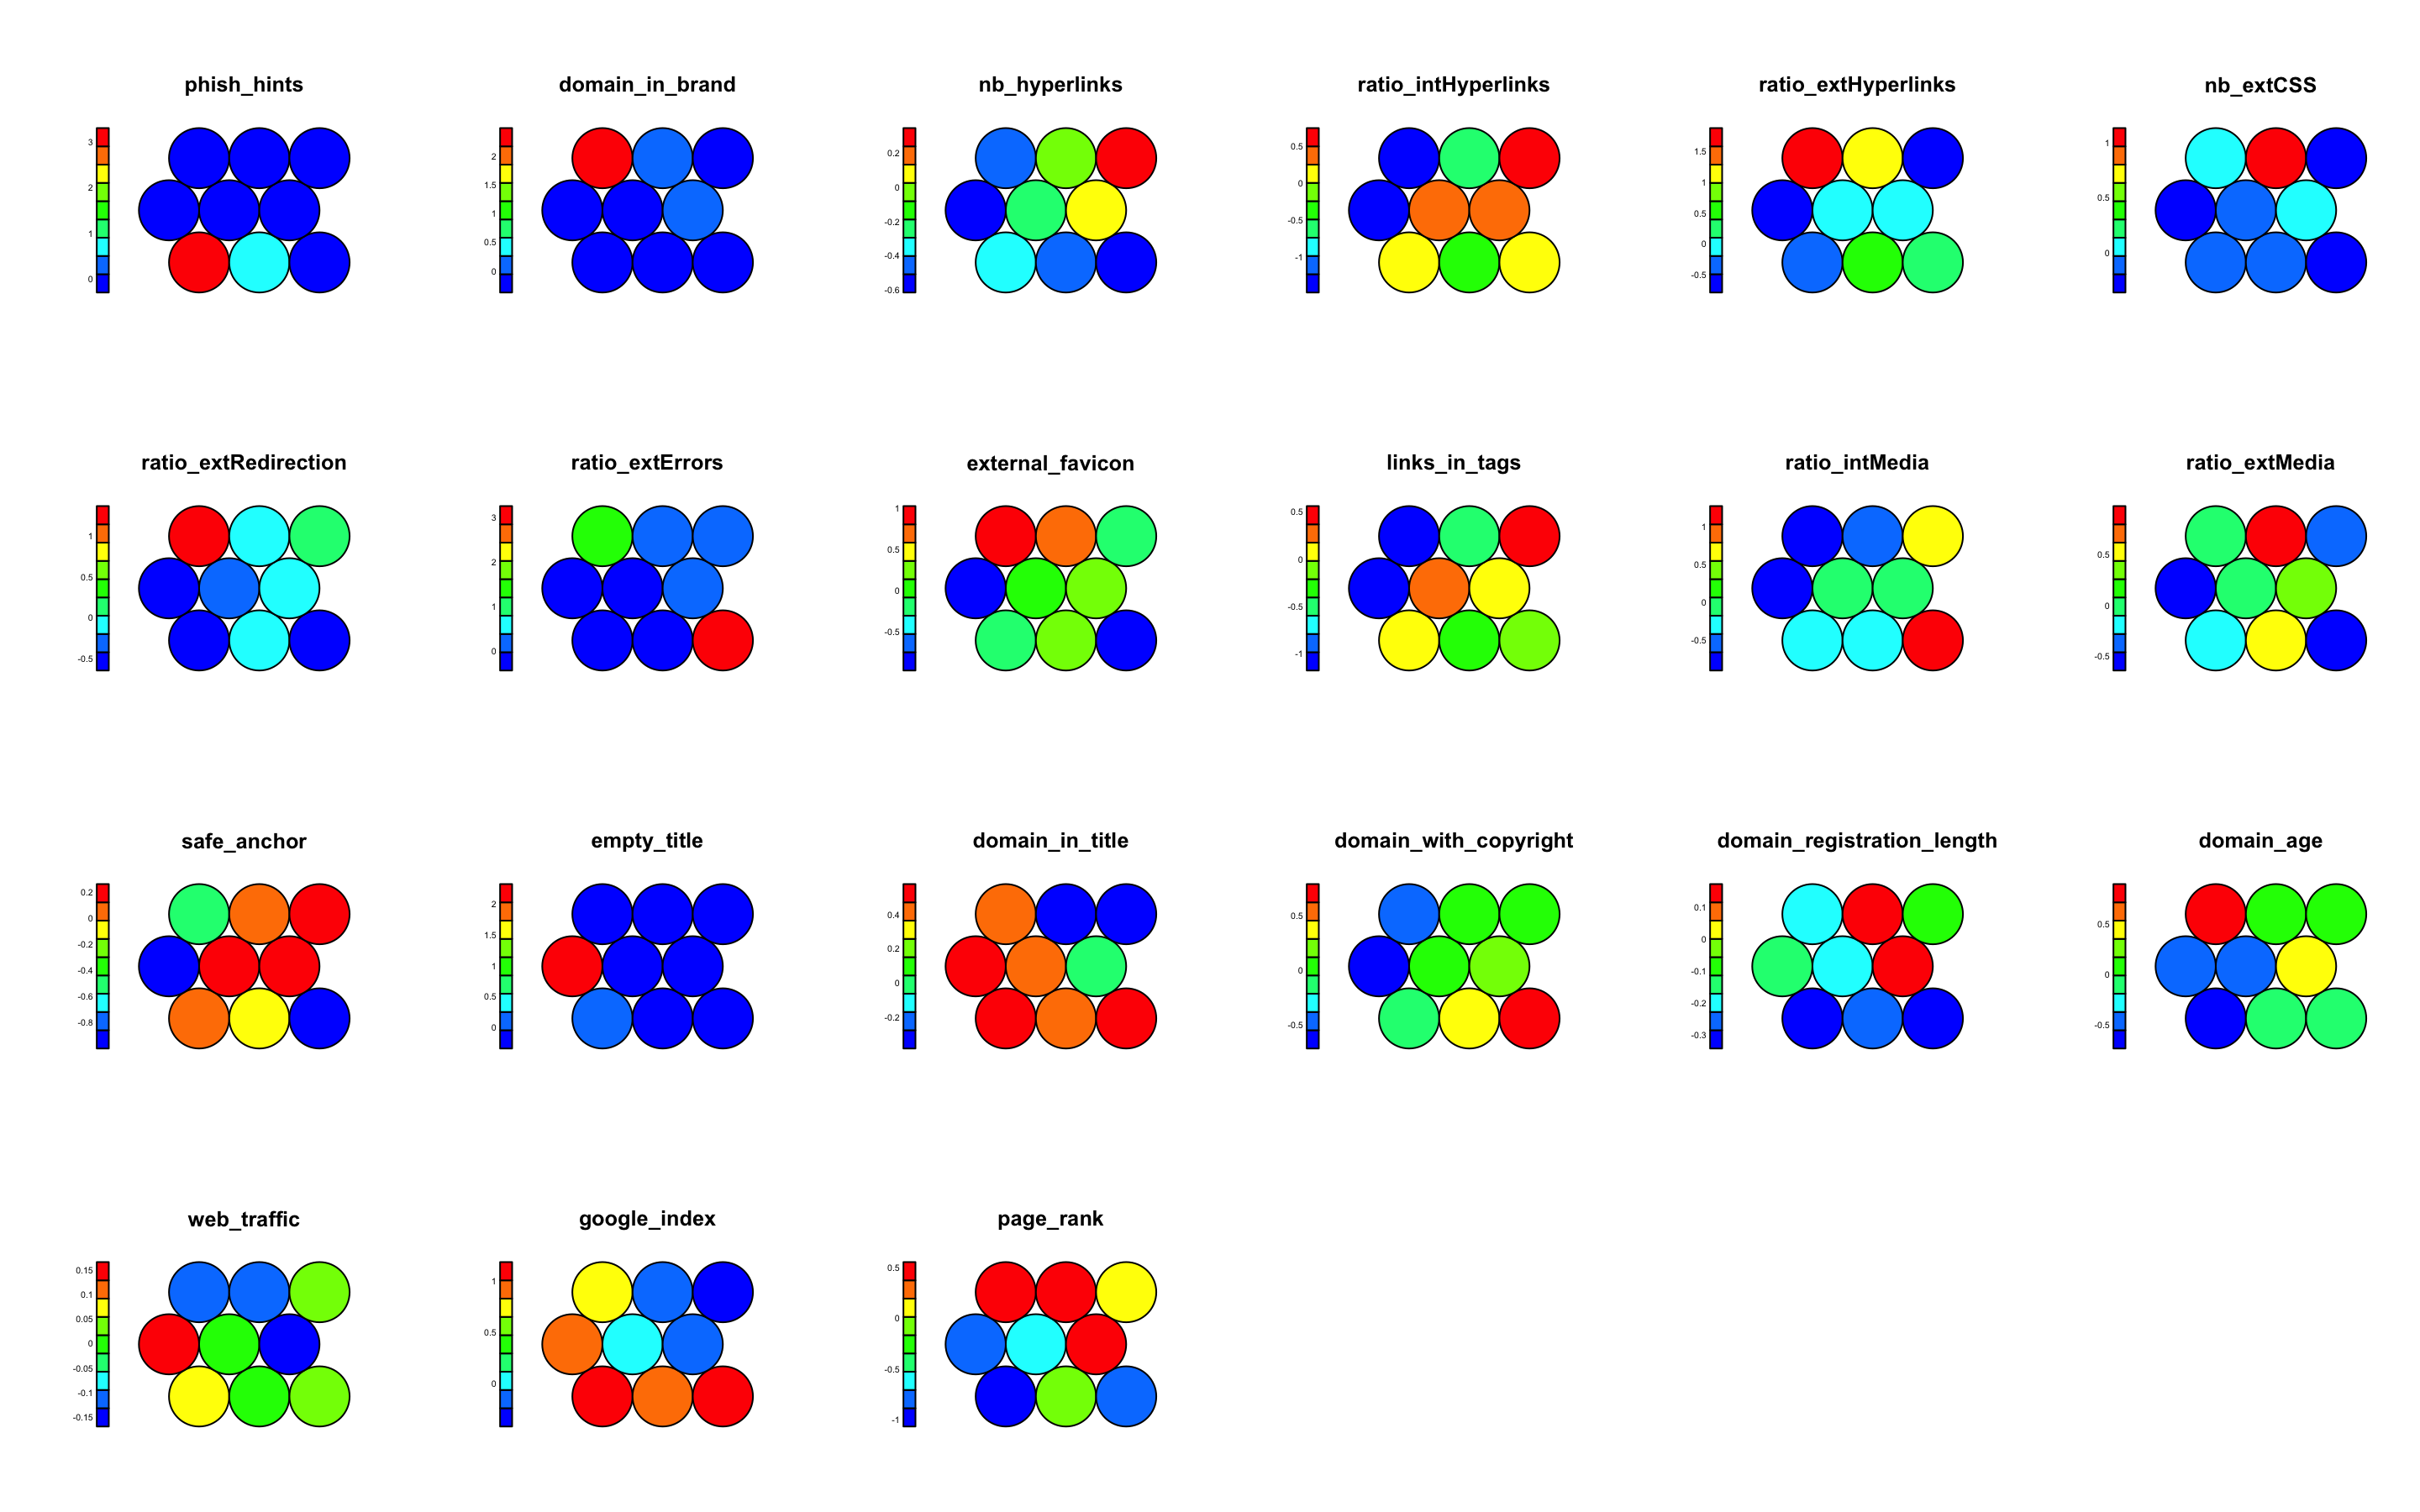
\includegraphics[width=1\textwidth]{maps2.png}
        \caption{Datos asociados a cada neurona según la variable}
        \label{fig:maps.png}
      \end{figure}

      \begin{figure}[H]
        \centering
        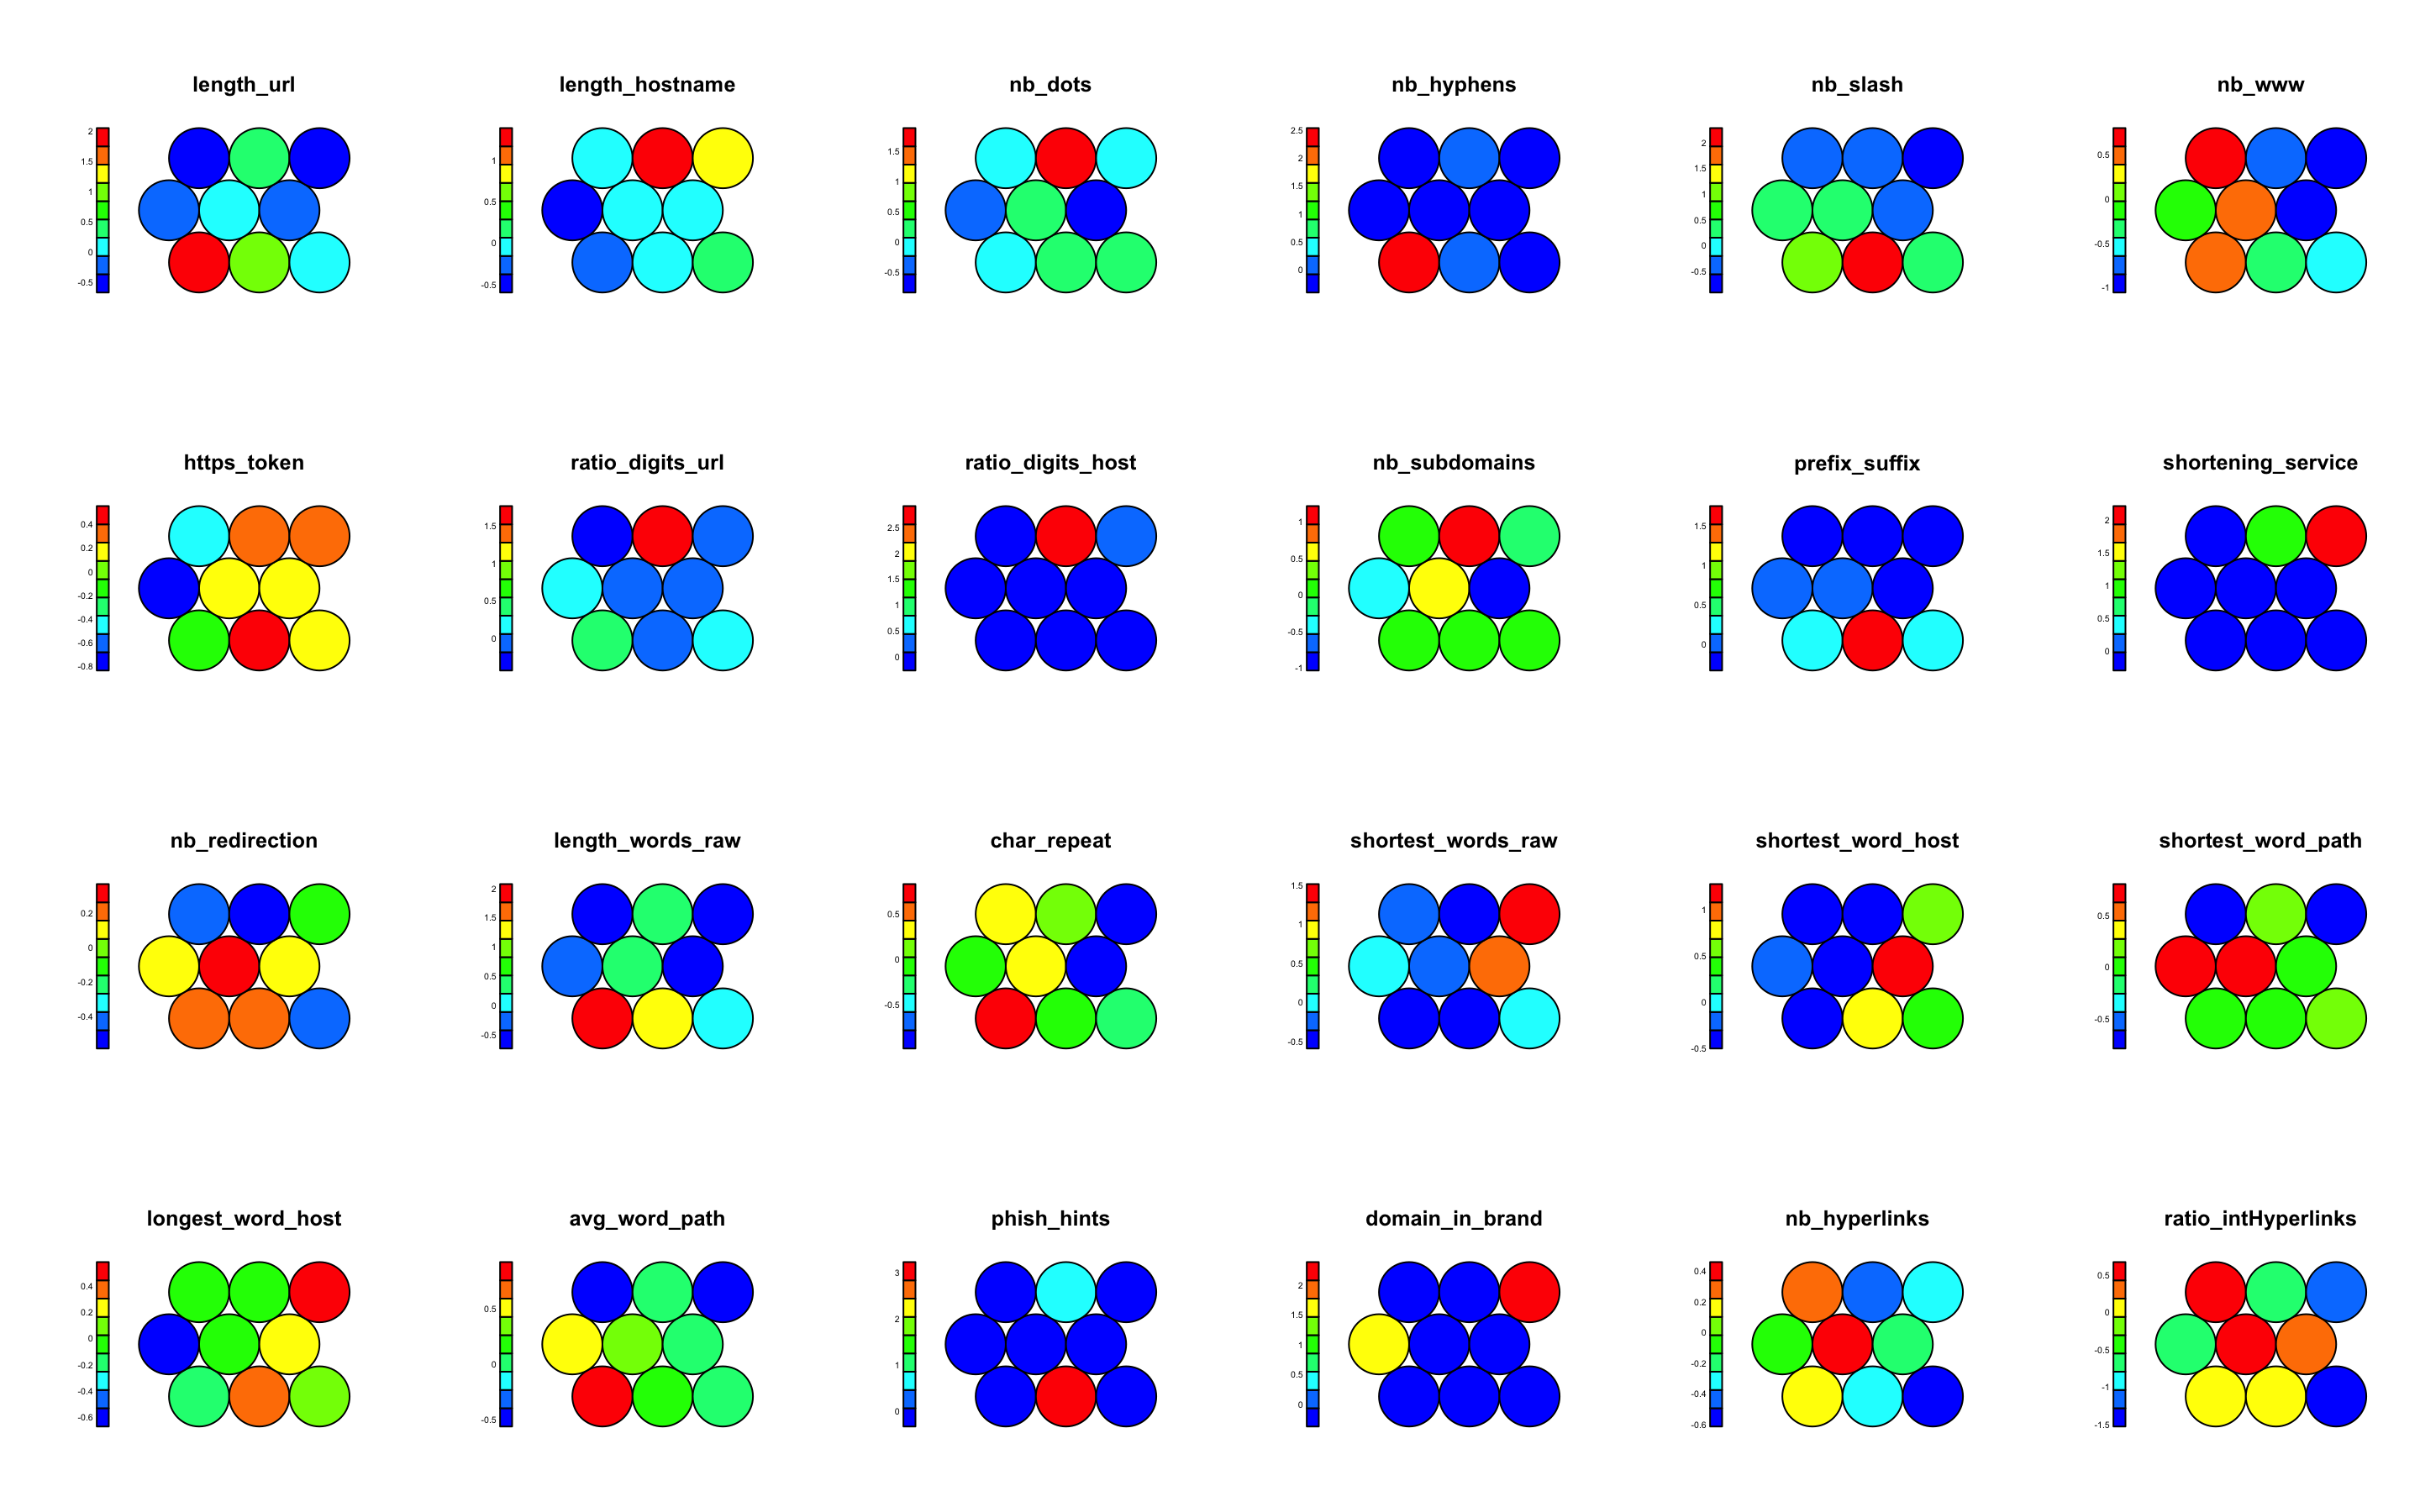
\includegraphics[width=1\textwidth]{maps1_nr.png}
        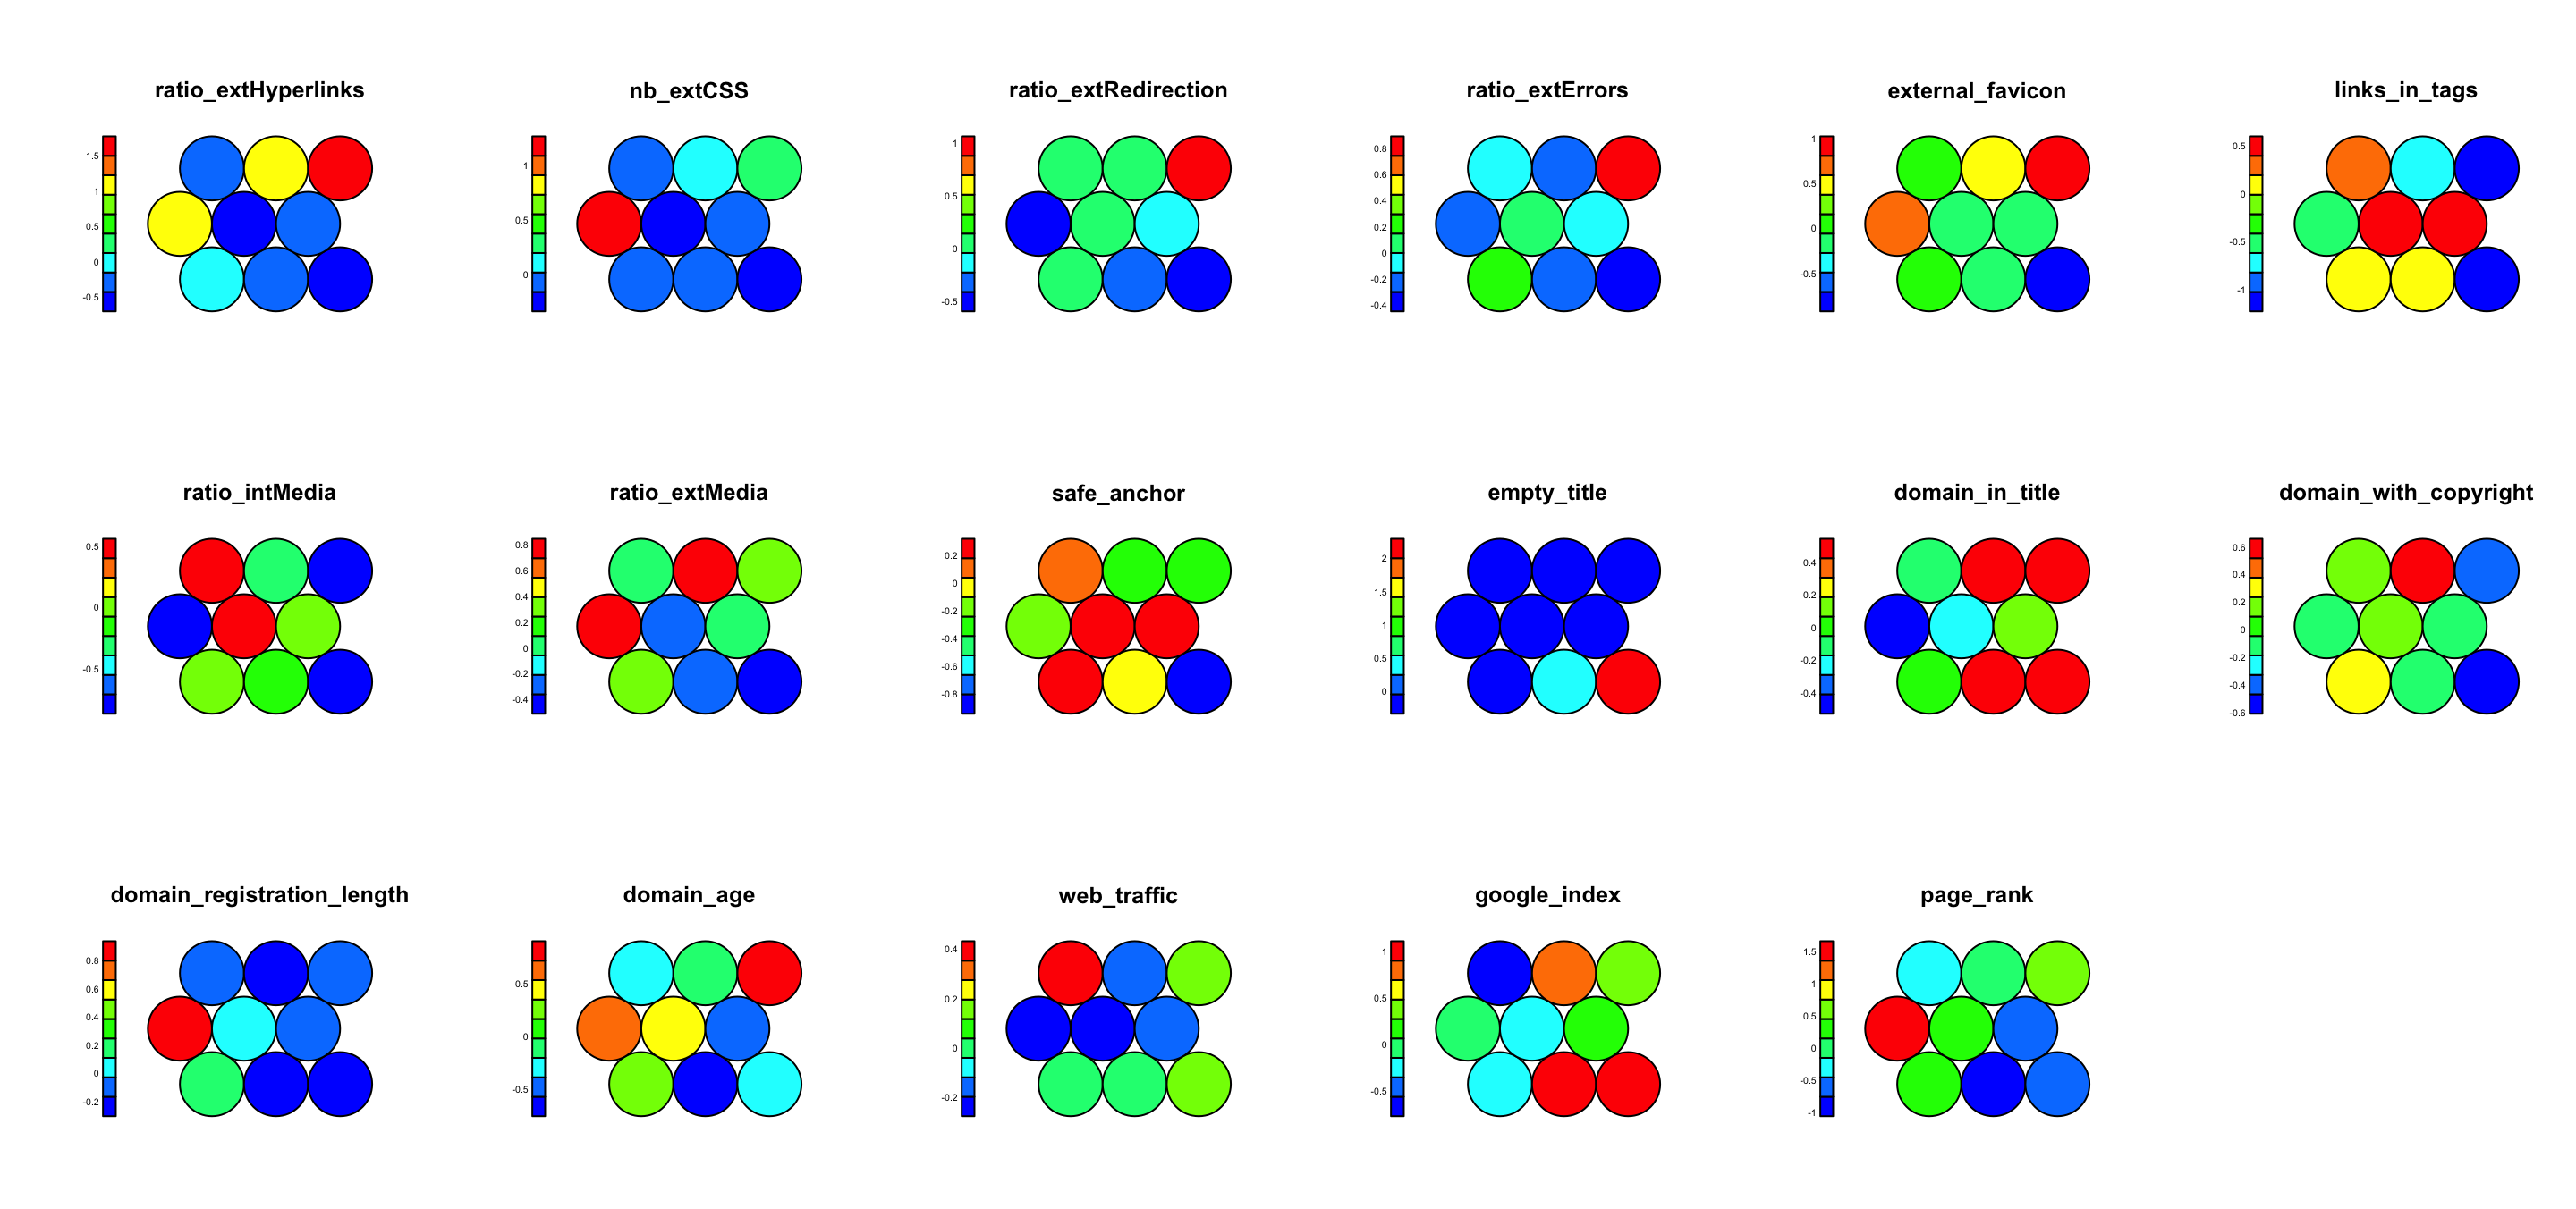
\includegraphics[width=1\textwidth]{maps2_nr.png}
        \caption{Datos asociados a cada neurona según la variable (sin redundancias)}
        \label{fig:maps_nr.png}
      \end{figure}

      Una vez obtenido el modelo, se realiza un \clustering\ jerárquico sobre los patrones descubiertos en las neuronas. Indicando un número de $2$ \clusters\ se obtiene la \figref{cluster_som.png}.

      Este modelo es difícil de analizar, ya que no proporciona demasiada información sobre los datos en el sentido de que los grupos formados no tienen una explicación clara, al igual que ocurría con \clustering\ jerárquico y con \kmeans.

      \figcaption{cluster_som.png}{\Clustering\ de los patrones descubiertos por cada neurona}{1}

    \subsection{Modelo supervisado}

      En este apartado se utiliza el mismo algoritmo de mapas de Kohonen y los mismos parámetros, pero en este caso el algoritmo conoce la clase a la que corresponden las observaciones para realizar el proceso de aprendizaje.

      Una característica de los mapas auto-organizados es que, como su propio nombre indica, los datos asociados a cada neurona tienden a agruparse en el mapa según su similitud. Esto puede verse en la \figref{classes_som.png}, donde se ve cómo las clases de tipo $1$ (URL legítimas) están separadas de las clases de tipo $2$ (URL con \phishing).

      \figcaption{classes_som.png}{Clases de las observaciones asociadas a cada neurona}{1}

      A continuación, se presentan las matrices de confusión obtenidas para el conjunto de entrenamiento y para el conjunto de test. La precisión obtenida es del \SI{88.79}{\percent} en entrenamiento y del \SI{87.44}{\percent} en test.

      \begin{minted}[bgcolor=bgcolor]{text}
Train:
             Reference
Prediction   legitimate   phishing
legitimate         2413        138
phishing            320       1213

Test:
             Reference
Prediction   legitimate   phishing
legitimate          783         45
phishing            126        407
      \end{minted}

      Los resultados obtenidos son aceptables, aunque se podría obtener una precisión mayor mediante otro algoritmo o añadiendo mayor complejidad al mapa.

  \section{KNN}

    Otro modelo de clasificación que se puede utilizar es KNN (\textit{K-Nearest-Neighbours}). Se trata de un algoritmo que utiliza directamente el conjunto de entrenamiento para predecir la clase de los elementos que se introduzcan al modelo.

    Se utiliza un conjunto de entrenamiento que supone un \SI{75}{\percent} del \dataset\ y el resto se destina al conjunto de test. El valor de \textit{K} óptimo es de $5$, lo cual significa que el dato entrante al modelo se compara con los 5 elementos del conjunto de entrenamiento más cercanos (los vecinos) y se le otorga la clase mayoritaria de ese grupo. La distancia utilizada es la euclídea.

    Al introducir el conjunto de test, se obtiene la siguiente matriz de confusión, con una precisión del \SI{94.35}{\percent}:

    \begin{minted}[bgcolor=bgcolor]{text}
             Reference
Prediction   legitimate   phishing
legitimate          800         49
phishing             28        485
    \end{minted}

    Como puede verse, la clasificación mediante este modelo es bastante buena, ya que se consigue una precisión elevada y con un algoritmo que no es necesario entrenar.

  \section{Árboles de decisión}

    Siguiendo con la clasificación de las URL, se pretende ahora analizar varios modelos basados en árboles de decisión.

    En primer lugar, se realizan distintos árboles de tipo CART y C4.5 con los paquetes \texttt{rpart} y \texttt{C50}, respectivamente; y en segundo lugar, se construye un modelo mediante \texttt{randomForest}.

    \subsection{CART}

      Utilizando una proporción del \SI{75}{\percent} del \dataset\ para el conjunto de entrenamiento, se crea un primer árbol de decisión de CART sin ninguna restricción. El árbol resultante se muestra en la \figref{cart.png}.

      \figcaption{cart.png}{Árbol de decisión de CART}{1}

      A continuación, se muestran las matrices de confusión para el conjunto de entrenamiento y el conjunto de test:

      \begin{minted}[bgcolor=bgcolor]{text}
Train:
             Reference
Prediction   legitimate   phishing
legitimate         2422        167
phishing            129       1366

Test:
             Reference
Prediction   legitimate   phishing
legitimate          794         53
phishing             34        480
      \end{minted}

      Aunque las precisiones obtenidas son elevadas (\SI{92.75}{\percent} para entrenamiento y \SI{93.61}{\percent} para test), podría considerarse que el árbol tiene complejidad innecesaria. En la siguiente \figref{cart_cp.png} se muestra el error que obtiene el árbol en función del número de nodos (\textit{splits}) y del parámetro de coste-complejidad:

      \figcaption{cart_cp.png}{Evolución del error en función del número de nodos y del coste-complejidad}{1}

      Si se realiza una poda del árbol con un parámetro de coste-complejidad de $0.014$ se obtiene un árbol más sencillo:

      \figcaption{cart_pruned.png}{Árbol de decisión de CART podado}{1}

      En este caso, la precisión del modelo se reduce al \SI{91.41}{\percent} en entrenamiento y \SI{91.70}{\percent} en test.

      \begin{minted}[bgcolor=bgcolor]{text}
Train:
             Reference
Prediction   legitimate   phishing
  legitimate       2444      244
  phishing          107     1289

Test:
             Reference
Prediction   legitimate   phishing
legitimate          798         83
phishing             30        450
      \end{minted}

      A la vista del árbol de la \figref{cart_pruned.png}, parece que una variable importante es la de \texttt{google\_index}, ya que si la URL está listada en Google (\texttt{google\_index=0}), el árbol lo clasifica directamente como sitio web legítimo.

    \subsection{C4.5}

      En este apartado se implementa un árbol de decisión mediante el algoritmo C4.5, para realizar una comparación con el árbol de CART anterior.

      Utilizando el paquete \texttt{C50} de R con los parámetros por defecto (factor de confianza de $0.25$), se obtiene un árbol bastante complejo, ya que consta de $47$ hojas. Al ver los resultados de las matrices de confusión se concluye que el modelo está sobre-aprendiendo.

      \begin{minted}[bgcolor=bgcolor]{text}
Train:
             Reference
Prediction   legitimate   phishing
legitimate         2519         39
phishing             32       1494

Test:
             Reference
Prediction   legitimate   phishing
legitimate          805         26
phishing             23        507
      \end{minted}

      Aunque las precisiones obtenidas son del \SI{98.26}{\percent} y del \SI{96.4}{\percent} en entrenamiento y en test, es preferible utilizar el árbol de CART podado, puesto que es más simple y no contiene casos específicos como el modelo de C4.5.

    \subsection{\textit{Random forest}}

      Para este modelo se aprovecha que el propio algoritmo tiene un proceso de \textit{bootstrap} antes de crear cada árbol individual, de manera que no es necesario separar el \dataset\ en un conjunto de entrenamiento y uno de test.

      Como primer modelo, se usa el método \textit{bagging} mediante la función \texttt{randomForest} con $45$ predictores y $500$ árboles. Con este modelo se consigue un error \textit{out-of-bag} (OOB) del \SI{1.82}{\percent} (precisión del \SI{98.18}{\percent}).

      \begin{minted}[bgcolor=bgcolor]{text}
             Reference
Prediction   legitimate   phishing
legitimate         3335         44
phishing             55       2011
      \end{minted}

      Como se puede observar, este modelo es muy bueno. Aún así, se puede tratar de mejorarlo mediante el método de \textit{random forest}, es decir, sin utilizar todos los predictores disponibles ($45$). En la \figref{mtry.png} se muestra la evolución del error OOB en función del número de predictores utilizados, resultando $3$ predictores el número óptimo.

      \figcaption{mtry.png}{Evolución del error OOB en función del número de predictores}{1}

      Una vez elegido este parámetro, se ajusta el tamaño de los nodos del árbol. En la siguiente \figref{nodesize.png} se presenta una gráfica con la evolución del error OOB según el tamaño de los nodos. En este caso, el valor óptimo es $1$.

      \figcaption{nodesize.png}{Evolución del error OOB en función del tamaño de los nodos}{1}

      \figcaption{trees.png}{Evolución del error OOB en función del número de árboles}{1}

      \newpage

      Por último, se puede ajustar el número de árboles escogiendo aquel que obtiene menos error OOB. En la \figref{trees.png} se ve cómo cambia el error según el número de árboles. El error mínimo se obtiene con $141$ árboles.

      Una vez establecidos los parámetros, se crea el modelo de \textit{random forest} y se obtiene un error OOB del \SI{1.6}{\percent} (precisión del \SI{98.4}{\percent}) y la siguiente matriz de confusión:

      \begin{minted}[bgcolor=bgcolor]{text}
             Reference
Prediction   legitimate   phishing
legitimate         3340         39
phishing             48       2018
      \end{minted}

      Con este modelo se obtiene un desempeño muy bueno. Al estar basado en árboles de decisión sencillos, el sobre-aprendizaje no supone un problema relevante.

      Adicionalmente, se puede conocer la importancia de las variables del \dataset, como se muestra en la \figref{importance.png}. Como se ha visto anteriormente, las más importantes son \texttt{google\_index}, \texttt{page\_rank} y \texttt{nb\_hyperlinks} (variables que aparecen en el árbol de CART podado de la \figref{cart_pruned.png}).

      \figcaption{importance.png}{Importancia de las variables en el modelo \textit{random forest}}{1}

  \newpage

  \section{Perceptrón multicapa}

    El último análisis a realizar es el modelo de perceptrón multicapa, basado en redes neuronales. El algoritmo utilizado está en el paquete \texttt{neuralnet} de R, al cual es necesario indicarle el número de capas de la red, el número de neuronas por capa y el tipo de función de salida (lineal o sigmoidal).

    Después de realizar varios experimentos con estos parámetros, se ve que la mejor red neuronal se obtiene con dos capas de $6$ y $3$ neuronas (capa oculta y capa de salida, respectivamente). La función de activación de salida es lineal. Una representación de la red se puede ver en la siguiente \figref{nn.png}:

    \figcaption{nn.png}{Red neuronal implementada}{1}

    Aunque la variable de salida \texttt{status} es categórica, el perceptrón multicapa se ha implementado para dar como resultado una variable continua. Se trató de poner una salida categórica pero el algoritmo no lograba converger. Como remedio, la salida de la red neuronal se discretiza redondeando su valor al número entero más cercano.

    En la siguiente \figref{nn_test.png} se muestra la salida del perceptrón multicapa, sin redondear, para el conjunto de test. Puede verse cómo la gran mayoría de predicciones se encuentran muy cercanas a los valores $1$ y $2$ (correspondientes a URL legítimas y con \phishing, respectivamente), de manera que el redondeo no afecta notablemente al resultado.

    \figcaption{nn_test.png}{Representación de los datos reales y las predicciones}{1}

    Para analizar el comportamiento del modelo, se probó a predecir los datos del conjunto de entrenamiento, obteniendo una precisión del \SI{99.51}{\percent}. Para el conjunto de test, la precisión es del \SI{97.5}{\percent}. Las matrices de confusión para ambos conjuntos se muestran a continuación:

    \begin{minted}[bgcolor=bgcolor]{text}
Train:
             Reference
Prediction   legitimate   phishing
legitimate         2542         11
phishing              9       1521

Test:
             Reference
Prediction   legitimate   phishing
legitimate          810         16
phishing             18        518
      \end{minted}

      Con este modelo se obtiene una precisión muy alta, demostrando la gran capacidad de las redes perceptrón multicapa para clasificar observaciones de un \dataset.

  \newpage
  \section*{Conclusiones}
    \addcontentsline{toc}{section}{Conclusiones}

    Después de realizar los modelos de \ML\ anteriores, se puede concluir que los algoritmos de \clustering\ no son apropiados para el objetivo del análisis, ya que no parece que agrupen las observaciones según lo esperado.

    Respecto a los algoritmos de clasificación, estos sí son apropiados, ya que el objetivo del análisis es precisamente clasificar las URL según su tipo (legítima o de \phishing). Ordenados de mejor a peor precisión obtenida en predicción, los modelos utilizados son los siguientes:

    \begin{itemize}
      \item \textit{Random forest}
      \item Perceptrón multicapa
      \item Árbol de decisión C4.5
      \item KNN
      \item Árbol de decisión CART (podado)
      \item Mapas de Kohonen (modelo supervisado)
    \end{itemize}

    Si se pretendiera utilizar uno de estos modelos para analizar URL de Internet y detectar posibles ataques de \phishing, los mejores modelos serían \textit{random forest} y perceptrón multicapa, los cuales obtienen una precisión muy elevada.

    Una opción más conservativa podría ser utilizar KNN, ya que es un algoritmo que no requiere de entrenamiento previo y directamente compara los datos entrantes con los datos del modelo para determinar la clase resultante. Además, también obtiene una precisión elevada.

    También es importante mencionar que en las matrices de confusión obtenidas, no hay muchos falsos negativos (es decir, que el modelo clasifique como URL legítima cuando realmente contiene \phishing), que es uno de los aspectos a minimizar.

    Otra conclusión que se puede realizar es que la limpieza inicial realizada sobre el \dataset\ original no ha causado problemas al implementar los modelos, indicando que fue una decisión acertada.

  \newpage

  \section*{Anexo: \Script\ para caracterizar una URL}
    \addcontentsline{toc}{section}{Anexo: \Script\ para caracterizar una URL}

    En este apartado se indica cómo utilizar el \script\ desarrollado en Python para obtener las características de una lista de URL para poder introducirlas a los modelos generados anteriormente.

    Se pretende que el programa sea utilizado mediante línea de comandos como se muestra a continuación:

    \begin{minted}[bgcolor=bgcolor]{bash}
$ cd scripts
$ pip install -r requirements.txt
$ python url_features.py -f url.txt -o output.csv
Results written in output.csv
Time: 33.716389179229736 seconds
    \end{minted}

    En el archivo \texttt{url.txt}, indicado por el parámetro \texttt{-f}, han de especificarse las distintas URL a caracterizar en una lista, tal y como se muestra en el siguiente ejemplo:

    \begin{minted}[bgcolor=bgcolor]{text}
https://www.google.com/
https://www.youtube.com/
https://github.com/
    \end{minted}

    Cabe mencionar que las URL indicadas tienen que ser accesibles. Es probable que las URL que realmente contengan \phishing\ solamente sean accesibles durante un tiempo limitado. Por este motivo, si se toma una URL con \phishing\ del \dataset, el programa no podrá caracterizarla porque seguramente no esté disponible en Internet.

    El resultado obtenido para las URL accesibles se escribe en un archivo indicado por el parámetro \texttt{-o} en formato CSV (por defecto, \texttt{output.csv}).

    Una vez que se tiene este archivo CSV, se puede predecir el tipo de URL mediante los modelos construidos en R mediante las siguientes funciones:

    \begin{itemize}
      \item \texttt{predict\_using\_randomforest(file)}
      \item \texttt{predict\_using\_mlp(file)}
      \item \texttt{predict\_using\_C50(file)}
      \item \texttt{predict\_using\_knn(file)}
      \item \texttt{predict\_using\_rpart(file)}
      \item \texttt{predict\_using\_som(file)}
    \end{itemize}

    Por ejemplo, puede ejecutarse el modelo de \textit{random forest} y utilizar la función de predicción correspondiente desde la consola de comandos de RStudio:

    \newpage

    \begin{minted}[bgcolor=bgcolor]{r}
> predict_using_randomforest(file = 'scripts/output.csv')
                         url       status
1    https://www.google.com/   legitimate
2   https://www.youtube.com/   legitimate
3        https://github.com/   legitimate
    \end{minted}

    Finalmente, se obtienen los resultados predichos por el modelo de manera clara y sencilla.

\end{document}
